
\section{Considerações Iniciais}

Este capítulo apresenta uma abordagem conceitual da modernização de sistemas e os esforços do OMG para a realização de uma padronização em nível de modelo desses sistemas. O escopo do trabalho é delimitado e se discute especificadamente sobre Modernização Dirigida a Arquitetura (do inglês - \textit{Architecture-Driven Modernization} - ADM) e \textit{Knowledge Discovery metamodel} (KDM). ADM é o processo de modernização apoiado por modelos do OMG que utiliza os conceitos da MDE. Neste capítulo, são abordados os principais pontos dessa modernização, bem como é apresentada uma descrição mais detalhada do seu principal metamodelo, que é o KDM.

O capítulo está organizado da seguinte forma: na Seção~\ref{sec:modernizacaoOrientada_Arquitetura} é feita uma contextualização sobre a Modernização Dirigida à Arquitetura; na Seção~\ref{sec:knowledge_discovery_meta_model} o metamodelo KDM é apresentado; na Subseção~\ref{subsection:codePackage} é descrito o pacote \texttt{Code}; na Subseção~\ref{sec:actionPackage} é descrito o pacote \texttt{Action}; na Subseção~\ref{sec:structurePackage} é apresentado o pacote \texttt{Structure}; na Seção~\ref{sec:Ferramenta_de_apoio_KDM_capitulo} é mostrada uma ferramenta de apoio ao KDM e na Seção~\ref{sec:consideracoes_finais_capitutloADM_KDM} são discutidas as considerações finais do capítulo.

\section{Modernização Dirigida a Arquitetura}\label{sec:modernizacaoOrientada_Arquitetura}

O crescente interesse na MDE motivou o \sigla{OMG}{\textit{Object Management Group}} a lançar a iniciativa denominada Modernização Dirigida a Arquitetura (do inglês - \textit{Architecture-Driven Modernization} (ADM)), cujo objetivo foi estabelecer metamodelos padronizados para auxiliar todo o  processo da reengenharia de software. Tal iniciativa foi motivada devido ao alto número de projetos reengenharia de software que não obtiveram sucesso~\cite{Sneed_2005, Demeyer2}. Como resultado desse esforço os conceitos da ADM foram criados, os quais possuem como objetivo revitalizar/modernizar softwares existentes\footnote{No contexto desse documento softwares existentes e sistemas legados são utilizados de forma intercambiáveis} com a utilização de metamodelos padronizados empregando os princípios da abordagem Arquitetura Dirigida a Modelo (do inglês - \sigla{MDA}{\textit{Model-Driven Architecture}}) (ver Seção~\ref{Cap2_Sec2_Desenvolvimento_Dirigido_a_Modelos}). %No contexto da ADM, todos os modelos são homogêneos, permitindo assim a criação de transformações \textit{Model-To-Model} M2M 

Dentre os termos mais recentes relacionados à reengenharia de software, a ADM se destaca. De acordo com o OMG~\cite{OMG_OMG} o objetivo da ADM não é substituir o processo tradicional da reengenharia de software, pelo contrário, a ADM tem como objetivo auxiliar e melhorar o processo de reengenharia de software por meio da utilização dos princípios da MDA. A ADM consiste em uma adaptação do modelo de ferradura tipicamente conhecido em reengenharia de software (i.e, o modelo de ferradura, basicamente contém dois lados, esquerdo, direito e uma \aspas{ponte} ligando os dois lados). Na Figura~\ref{fig:horse_shoe} é apresentado o modelo de ferradura adaptado para a ADM. É importante observar que essa figura contém todas as fases e \aspas{palavras-chaves} tradicionais que são encontradas na reengenharia de software tradicional e em MDA, tais como: Modelo Especifico de Plataforma (do inglês - \textit{Platform-Specific Model} (PSM)), Modelo Independente de Plataforma (do inglês - \textit{Platform-Independent Model} (PIM)) e Modelo Computacional Independente (do inglês - \textit{Computation-Independent Model} (CIM)). As fases tradicionais da reengenharia de software adaptadas para a ADM são:


\begin{itemize}
 	\item \textbf{Engenharia Reversa}: Esta fase tem como entrada um sistema que será modernizado, posteriormente esse sistema é transformado em um PSM. Além disso, o PSM é utilizado como entrada para a geração do PIM, que no contexto dessa tese consiste em uma instância do metamodelo denominado KDM (ver Seção~\ref{sec:knowledge_discovery_meta_model}) que será explicado com mais detalhes posteriormente;
 	\item \textbf{Reestruturação}: Nesta fase um conjunto de reestruturação/refatoração pode ser aplicado sobre uma instância do metamodelo KDM por meio de transformações de modelo para modelo (do inglês - \sigla{M2M}{\emph{Model-To-Model}});
 	\item \textbf{Engenharia Avante}: Nesta fase um novo código-fonte do sistema modernizado é gerado automaticamente por meio de transformações de modelo para código (do inglês - \sigla{M2C}{\emph{Model-To-Code}}). 
 \end{itemize} 

 \begin{figure}[htb]
 \caption{Modelo de ferradura adaptada para a ADM}
 \label{fig:horse_shoe}
 \centering
 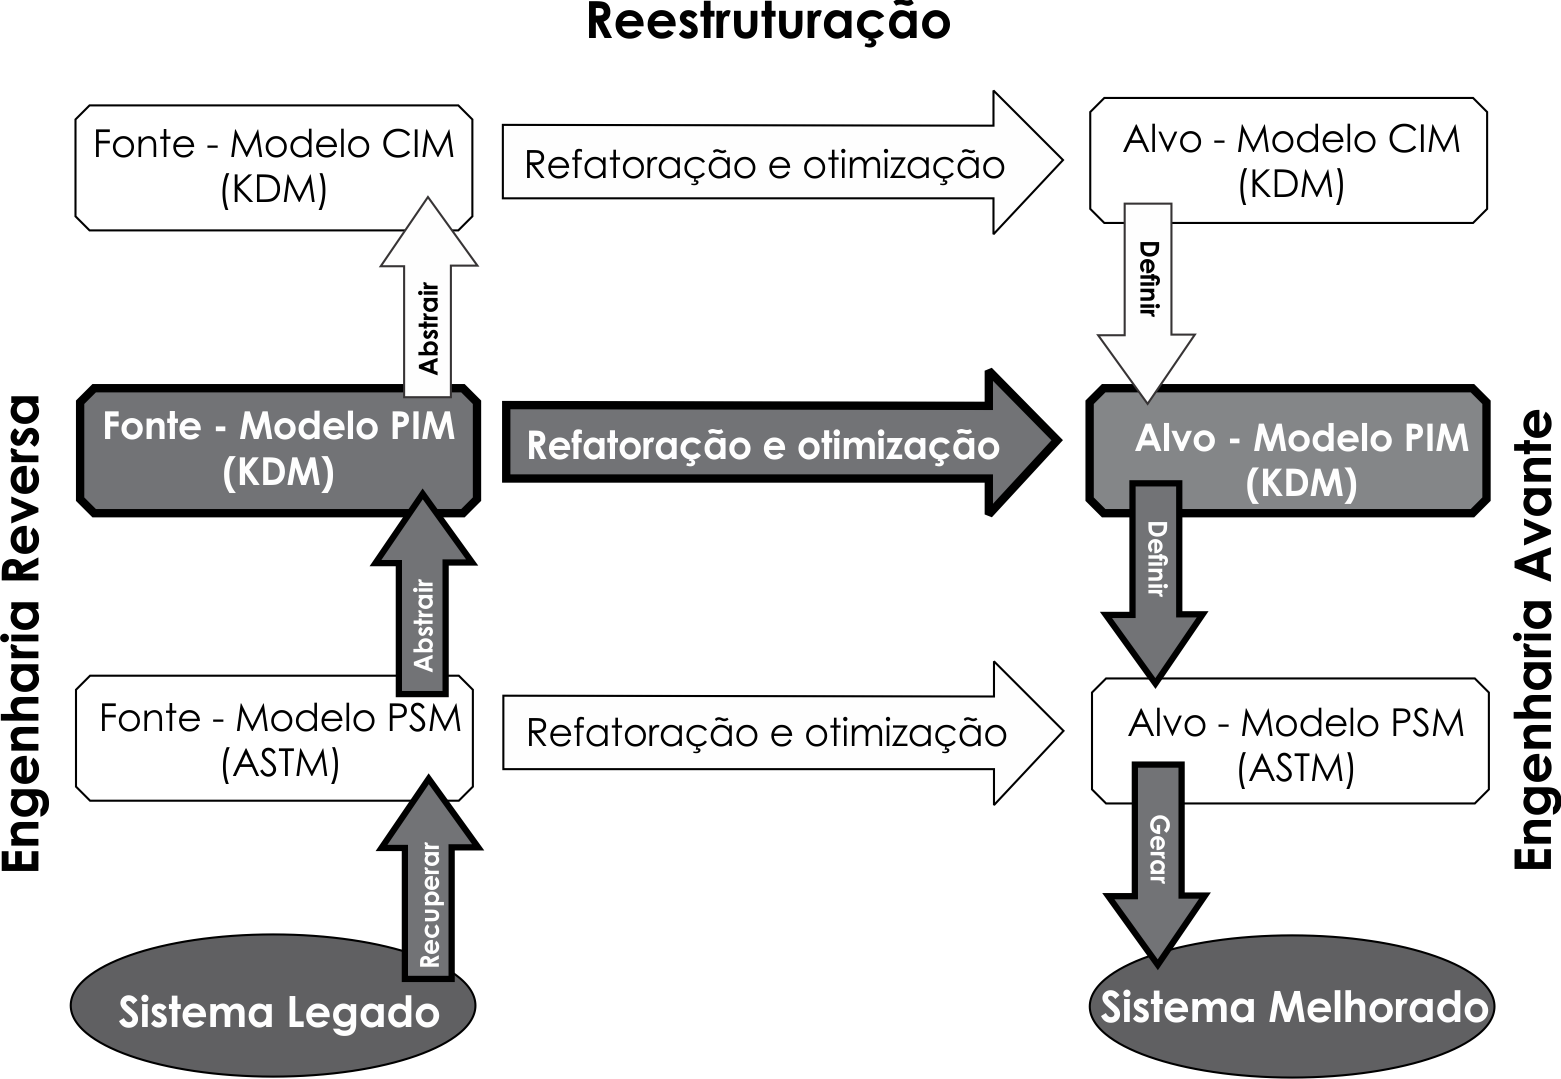
\includegraphics[scale=0.78]{images/modelo-ferradura.png}
 \fadaptada{ADM:OMG}
\end{figure}

Durante o processo da ADM todos os modelos (i.e., PSM, PIM e CIM) podem estabelecer transformações/refatorações entre si, como ilustrado na Figura~\ref{fig:horse_shoe}. Geralmente tais transformações são executadas por meio de linguagens de transformações. Como salientado no Capítulo~\ref{chapter:fundamentacao_teorica}, Seção~\ref{sec:transformacoes_de_modelos} usualmente essas transformações são implementadas utilizando diferentes linguagens de transformações que podem ser declarativas, imperativas ou híbridas. 

É importante também destacar que a ADM não tem como intuito apenas seguir todos os princípios da abordagem MDA~\cite{ADM:OMG}. Um dos principais objetivos da ADM é definir um conjunto de metamodelos, padronizados, para lidar com diferentes desafios que são encontrados hoje em dia na reengenharia de software. Dessa forma, em Novembro de 2003, a \sigla{ADMTF}{\textit{Architecture-Driven Modernization Task Force}} criou uma \sigla{RFP}{\textit{Request-for-Proposal}} que por sua vez descrevia um conjunto de metamodelos. Tais metamodelos são: (\textit{i}) Knowledge Discovery Metamodel (KDM), maiores informações sobre esse metamodelo é apresentado na seção~\ref{sec:knowledge_discovery_meta_model}, (\textit{ii}) \sigla{SMM}{\textit{Structured Metrics metamodel}} que é um metamodelo para representar e definir métricas e resultados de medições, (\textit{iii}) \sigla{ADMPR}{\textit{ADM Pattern Recognition}}, que facilita a busca de padrões em um software, (\textit{iv}) \sigla{ADMVS}{\textit{ADM Visualization Specification}}, que tem como objetivo representar visualmente metadados de uma aplicação representada em KDM, (\textit{v}) \sigla{ADMRS}{\textit{ADM Refactoring Specification}}, que almeja definir um metamodelo padronizado para especificar e definir refatorações utilizando outros metamodelos da ADM, como por exemplo o KDM. O estado atual de cada metamodelo pode ser visto na Tabela~\ref{tab:todos_os_meta_modelos_da_ADM}~\cite{ADM:OMG}. Como observado nessa tabela, alguns metamodelos ainda encontram-se em fase de desenvolvimento e outros já foram finalizadas e disponíveis pelo OMG.

% Please add the following required packages to your document preamble:
% \usepackage{multirow}
\begin{table}[]
\centering
\caption{Estado atual dos metamodelos da ADM.}
\label{tab:todos_os_meta_modelos_da_ADM}
\begin{tabular}{|l|l|l|l|}
\hline
\multicolumn{1}{|c|}{Metamodelo}                                         & \multicolumn{1}{c|}{Situação}           & \multicolumn{1}{c|}{Versão} & \multicolumn{1}{c|}{Data}          \\ \hline
\textit{ADM Pattern Recognition} (ADMPR)                     & Em desenvolvimento &\multicolumn{1}{c|}{\textemdash}&\multicolumn{1}{c|}{\textemdash}\\ \hline
\textit{ADM Refactoring Specification} (ADMRS)               & Em desenvolvimento &\multicolumn{1}{c|}{\textemdash}&\multicolumn{1}{c|}{\textemdash}\\ \hline
\textit{ADM Visualization Specification} (ADMVS)             & Em desenvolvimento &\multicolumn{1}{c|}{\textemdash}&\multicolumn{1}{c|}{\textemdash}\\ \hline
\sigla{ASTM}{\textit{Abstract Syntax Tree Metamodel}}               & \multicolumn{1}{c|}{Disponível}         & \multicolumn{1}{c|}{1.0}    & \multicolumn{1}{c|}{2011}  \\ \hline
\textit{Knowledge Discovery Metamodel} (KDM)                 & \multicolumn{1}{c|}{Disponível}         & \multicolumn{1}{c|}{1.3}    & \multicolumn{1}{c|}{2011}   \\ \hline
\multirow{2}{*}{\textit{Structured Metrics Metamodel} (SMM)} & \multicolumn{1}{c|}{Disponível}         & \multicolumn{1}{c|}{1.0}    & \multicolumn{1}{c|}{2012}  \\ \cline{2-4} 
                                                    & Em desenvolvimento & \multicolumn{1}{c|}{1.1}    & \multicolumn{1}{c|}{2013} \\ \hline
\end{tabular}
\end{table}

É importante destacar que a abordagem proposta nesta Tese, se concentra no metamodelo KDM. Consequentemente, é de suma importância o entendimento desse metamodelo, por isso, esse metamodelo é mais detalhado neste capítulo.
KDM é um metamodelo que pode ser utilizado para representar todos os artefatos de um determinado software existente, por exemplo, o KDM contém metaclasses especificas para representar desde de código-fonte até a arquitetura de um determinado software. O KDM é um metamodelo de representação intermediária comum para sistemas existentes e seus ambientes operacionais. Utilizando esse metamodelo para sistemas existentes é possível trocar representações do sistema em modelo entre plataformas e linguagens com a finalidade de analisar, padronizar e transformar/refatorar os sistemas existentes~\cite{ADM:OMG}. 

A ideia por trás do KDM é que a comunidade comece a criar analisadores sintáticos (do inglês - \textit{parsers}) para diferentes linguagens de programação, que transforme os códigos-fontes em instâncias do metamodelo KDM. Como resultado, qualquer técnica, ferramenta e abordagem que utilize o KDM como o artefato de entrada pode ser considerado uma técnicas, ferramenta e/ou abordagem independente de linguagem e de plataforma. Por exemplo, um catálogo de refatoração para o KDM~\cite{durelli_catalogo, durelli_VEM_ferramenta} pode ser utilizado para refatorar vários sistemas independentemente da linguagem de programação. Maiores informações sobre o KDM, bem como seus pacotes, metaclasses e metarelacionamentos são apresentados a seguir.

\section{Knowledge Discovery Metamodel (KDM)}
\label{sec:knowledge_discovery_meta_model}

\sigla{KDM}{Knowledge Discovery Metamodel} é um metamodelo para representar existentes artefatos de software, seus elementos, associações, e ambientes operacionais. O KDM tem como principal objetivo permitir que engenheiros de software criem ferramentas para auxiliar a modernização de software que sejam independente de plataforma e linguagem~\cite{KDM:specification, PerezCastillo:2011jo, ADMCHAPTERR}. Além disso, o KDM facilita e assegura a interoperabilidade e troca de dados entre diferentes ferramentas. 

Um problema tradicional facilmente identificado em várias ferramentas que lidam com a reengenharia de software é que tais ferramentas analisam diversos artefatos de um determinado software (por exemplo, código-fonte, banco de dados, \textit{scripts}, etc.) para obter conhecimentos explícitos com o intuito de realizar transformações/refatorações~\cite{rosenberg, Canfora2011}. Como consequência cada ferramenta gera e analisa tais conhecimentos de forma implícita. Assim, os conhecimentos gerados são restritos a uma especifica linguagem de programação, e/ou a uma plataforma. Como resultado tais restrições podem criar dificuldades com relação a interoperabilidade entre diferentes ferramentas. O KDM fornece uma estrutura que tem com objetivo facilitar a troca de dados entre diversas ferramentas. Além disso, o KDM possui um conjunto de metaclasse e uma estrutura padronizada que fornece meios para especificar desde artefatos físicos até artefatos lógicos de um determinado sistema de software. Em virtude dessa padronização, todas as técnicas/abordagem/ferramentas que utilizam o KDM como entrada pode ser considerada independente de plataforma e linguagem, aumentando assim, a interoperabilidade e o reúso. Em 2012 o KDM tornou-se \sigla{ISO}{\emph{International Standards Organization}}~\cite{KDM:ISO} como uma estrutura que facilita a troca de dados entre as diversas ferramentas. O KDM é definido via \sigla{MOF}{\emph{Meta-Object Facility}}~\cite{MOF} e estabelece o formato de troca de dados via \sigla{XMI}{\emph{XML Metadata Interchange}}, o qual é denominado KDM XMI \emph{schema}.


Pode-se sumarizar os principais objetivos do KDM como~\cite{ADM:OMG}: (\textit{i}) KDM representa artefatos de um sistema legado como entidades, relacionamentos e atributos; (\textit{ii}) KDM suporta uma variedade de plataforma e linguagem; (\textit{iii}) KDM define uma terminologia unificada para artefatos de sistemas legados; (\textit{iv}) KDM representa estruturas lógicas e físicas de sistemas legados; (\textit{v}) KDM permite a modificação/refatoração de sistemas legados utilizando os princípios da MDA; (\textit{vi}) KDM facilita o rastreamento de mudança entre artefatos; (\textit{vii}) KDM facilita a sincronização de estruturas lógicas e físicas de um determinado sistema legado; (\textit{viii}) KDM contém metaclasses para representar desde código-fonte até metaclasses para representar elementos arquiteturais de um determinado sistema legado.

%\begin{itemize}
	%\item KDM representa artefatos de um sistema legado como entidades, relacionamentos e atributos;
	%\item KDM suporta uma  variedade de plataforma e linguagem;
%	\item KDM define uma terminologia unificada para artefatos de sistemas legados;
	%\item KDM representa estruturas lógicas e físicas de sistemas legados;
	%\item KDM permite a modificação/refatoração de sistemas legados utilizando os princípios da MDA;
	%\item KDM facilita o rastreamento de mudança entre artefatos;
	%\item KDM facilita a sincronização de estruturas lógicas e físicas de um determinado sistema legado;
	%\item KDM contém metaclasses para representar desde código-fonte até metaclasses para representar elementos arquiteturais de um determinado sistema legado.
%\end{itemize}

De acordo com~\citeonline{PerezCastillo:2011jo} o KDM possui o objetivo de cobrir um amplo escopo, para abranger um conjunto diversificado de aplicações, plataformas e linguagens de programação. Um dos principais objetivos do KDM é fornecer a capacidade de troca de metadados entre diversas ferramentas e, assim, facilitar a cooperação entre fornecedores para integrar e aumentar a interoperabilidade de diferentes abordagens, técnicas, algoritmos, etc. A fim de alcançar essa interoperabilidade e, especialmente, a integração de informações sobre diferentes facetas de um determinado sistema a partir de múltiplas ferramentas, o KDM define vários níveis de conformidade, aumentando assim a probabilidade de que duas ou mais ferramentas apoiaram o mesmo metamodelo. Além disso, o KDM também é estruturado de forma modular, seguindo o princípio da separação de interesse, com a capacidade de representar partes heterogêneas de um sistema. A separação de interesses no contexto do metamodelo KDM é alcançada por meio de pacotes, como apresentado na Figura~\ref{kdm:domain}. Cada pacote está em um nível de conformidade e possui o objetivo de definir um ponto de vista arquitetural do sistema. Em outras palavras, cada pacote do KDM constitui uma determinada ontologia para descrever e representar a grande maioria dos artefatos de sistemas de software existentes. Por exemplo, os pacotes \texttt{Code} e \texttt{Action} contêm metaclasses que representam o código-fonte de um sistema, tais como, variáveis, procedimentos/métodos/funções, chamadas para métodos, etc. Similarmente o pacote \texttt{Structure} contém metaclasses para representar elementos arquiteturais do sistema, tais como, componentes, camadas, subcomponentes, etc. O pacote \texttt{Conceptual} possui  metaclasses para definir regras de negócio do sistema.


\begin{figure}[htb]
 \caption{Pacotes e nível de conformidade do metamodelo KDM.}
 \label{kdm:domain}
 \centering
 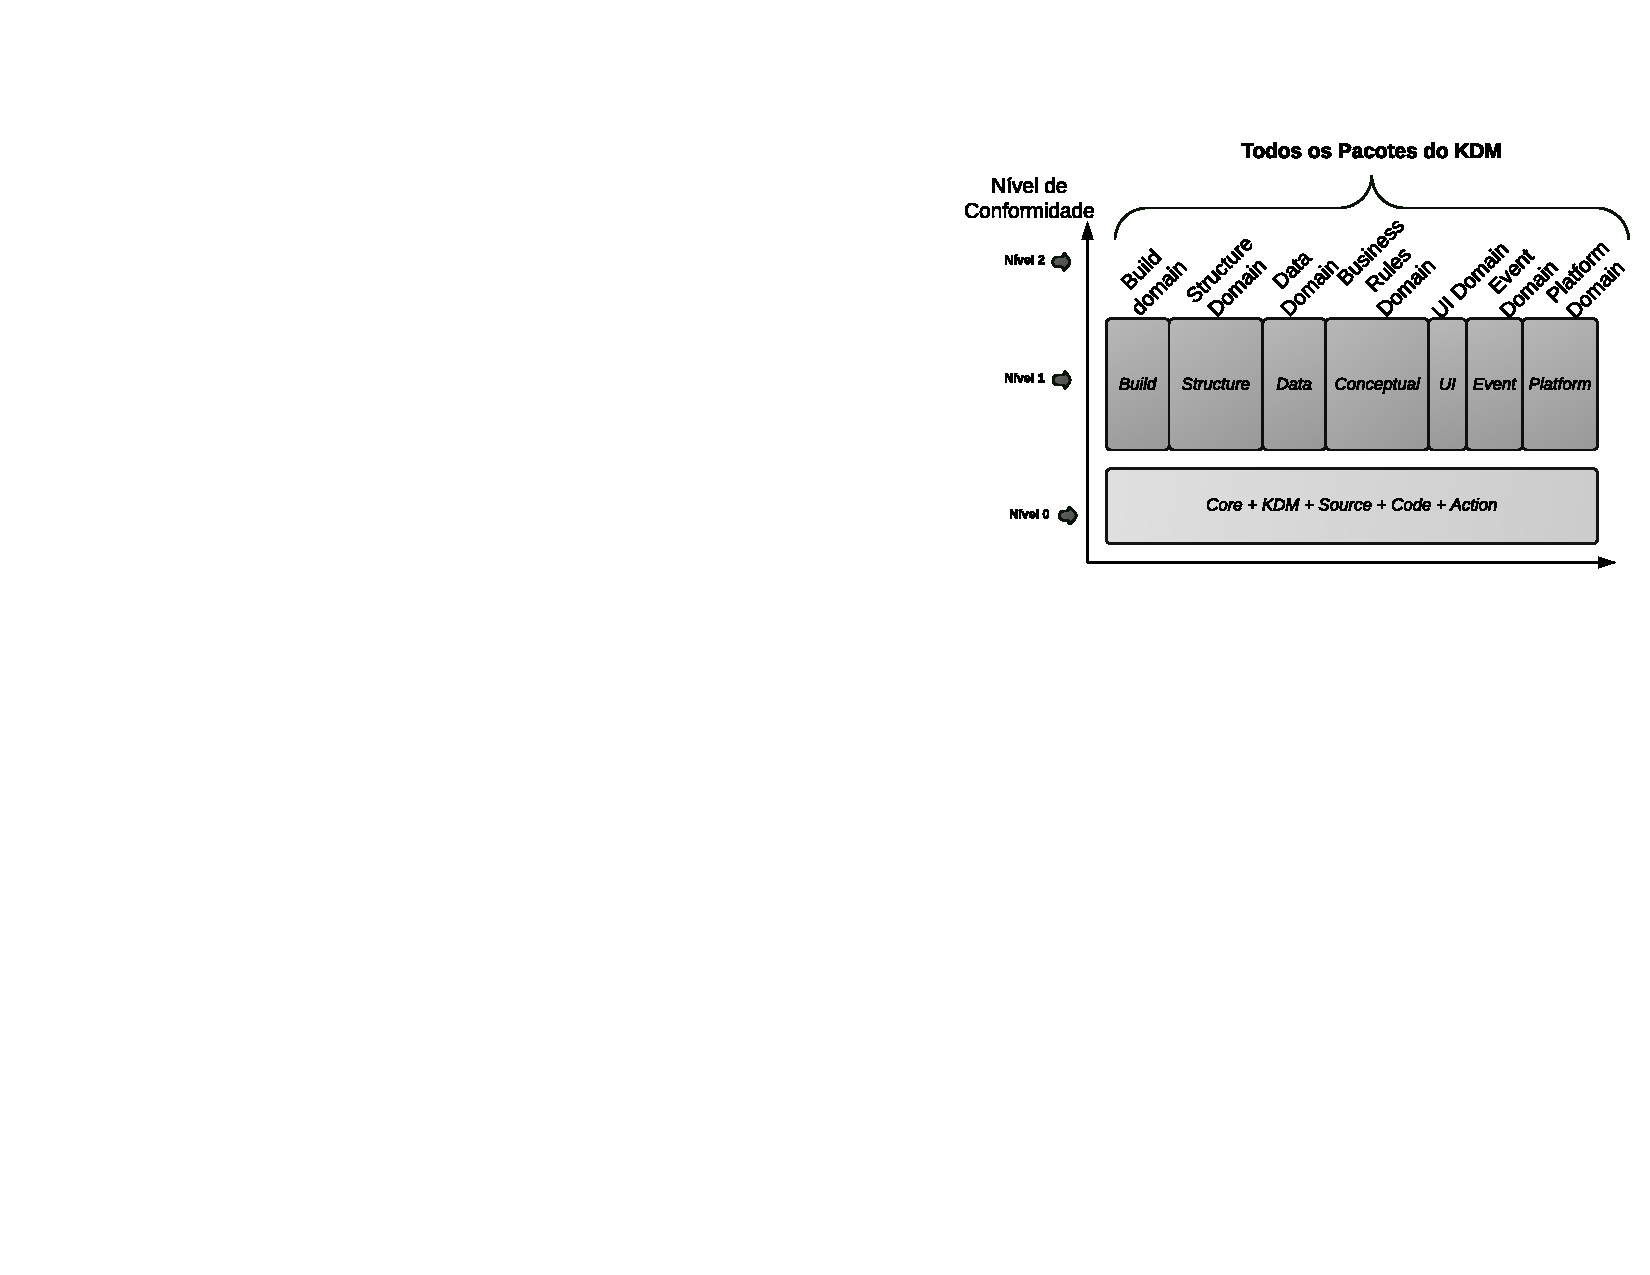
\includegraphics[scale=1]{images/kdmLevels_pacotes.pdf}
 \fadaptada{KDM:specification}
\end{figure}

Da perspectiva de um engenheiro de modernização, essa separação de interesse do KDM, por meio de pacote, significa que o engenheiro só precisa se preocupar com os pacotes do KDM que considerar necessários para as suas atividades de modernização, por exemplo, uma determinada abordagem pode necessitar apenas do pacote \texttt{Code} e \texttt{Action}, enquanto uma outra abordagem pode utilizar apenas o pacote responsável por definir elementos arquiteturais. Se essas abordagens forem evoluídas ao longo do tempo e necessitarem de outros pacotes do KDM, pacotes podem ser adicionados ao repertório da abordagem/ferramenta, conforme necessário.

Como observado na Figura~\ref{kdm:domain} o KDM possui três níveis de conformidade, nível 0, nível 1 e nível 2. Informações sobre cada nível são apresentadas a seguir:

\begin{itemize}
    \item \textbf{Nível 0}: nesse nível de conformidade são definidos os seguintes pacotes do KDM: (\textit{i})     \texttt{Core}, (\textit{ii}) \texttt{kdm}, (\textit{iii}) \texttt{Source}, (\textit{iv}) \texttt{Code} e (\textit{v}) \texttt{Action}. Esse nível de conformidade representa um denominador comum que pode servir como uma base para a interoperabilidade entre diferentes categorias de ferramentas que utilizem o metamodelo KDM. Para que uma ferramenta esteja em conformidade com o \textbf{Nível 0} ela deve fornecer completo suporte para todas as metaclasses que foram definidas nos pacotes \texttt{Core}, \texttt{kdm}, \texttt{Source}, \texttt{Code} e \texttt{Action};
    \item \textbf{Nível 1}: nesse nível os pacotes definidos no \textbf{Nível 0} são estendidos para representar outros artefatos de um determinado sistema. Esse nível define os seguintes pacotes: (\textit{i}) \texttt{Build}, (\textit{ii}) \texttt{Structure}, (\textit{iii}) \texttt{Data}, (\textit{iv}) \texttt{Conceptual}, (\textit{v}) \texttt{UI}, (\textit{vi}) \texttt{Event} e (\textit{vii}) \texttt{Platform}. Para que uma ferramenta esteja em conformidade com o \textbf{Nível 1} ela deve fornecer suporte para todos os pacotes do \textbf{Nível 0} pelo menos um do pacotes do Nível 1;
    \item \textbf{Nível 2}: esse nível é a união de todos os pacotes definidos no nível anterior. Para que uma ferramenta esteja em conformidade com o \textbf{Nível 2} ela deve fornecer suporte para todos os pacotes do \textbf{Nível 1} e pelo menos um do \textbf{Nível 2}.
\end{itemize}


Todos os pacotes do metamodelo KDM apresentado na Figura~\ref{kdm:domain} são organizados em quatro camadas de abstração. As camadas de abstração são: (\textit{i}) \sigla{CI}{Camada de Infraestrutura}: do inglês \textit{Infrastructure Layer}; (\textit{ii}) \sigla{CEP}{Camada de Elementos de Programa}: do inglês \textit{Program Elements Layer}; (\textit{iii}) \sigla{CRTE}{Camada de Recurso de Tempo de Execução}: do inglês \textit{Runtime Resource Layer}; (\textit{iv}) \sigla{CA}{Camada de Abstração}: do inglês \textit{Abstraction Layer}. Essas quatro camadas estão apresentadas esquematicamente na Figura~\ref{fig:kdm_layer}.

%\begin{itemize}
    %\item \sigla{CI}{Camada de Infraestrutura}: do inglês \textit{Infrastructure Layer};
    %\item \sigla{CEP}{Camada de Elementos de Programa}: do inglês \textit{Program Elements Layer};
    %\item \sigla{CRTE}{Camada de Recurso de Tempo de Execução}: do inglês \textit{Runtime Resource Layer};
    %\item \sigla{CA}{Camada de Abstração}: do inglês \textit{Abstraction Layer}.
%\end{itemize}


%(\textit{i}) \sigla{CI}{Camada de Infraestrutura} (do inglês \textit{Infrastructure Layer}), (\textit{ii}) \sigla{CEP}{Camada de Elementos de Programa} (do inglês \textit{Program Elements Layer}), (\textit{iii}) \sigla{CRTE}{Camada de Recurso de Tempo de Execução} (do inglês \textit{Runtime Resource Layer}) e (\textit{iv} ) \sigla{CA}{Camada de Abstração} (do inglês \textit{Abstraction Layer}). 

%Cada camada é posteriormente organizada em pacotes, como pode ser observado na Figura~\ref{fig:kdm_layer}. Por sua vez, cada pacote define um conjunto de metaclasses cujo propósito é representar o conhecimento de específicos artefatos de um determinado sistema. 

%
\begin{figure}[htb]
 \caption{Camadas e pacotes do KDM.}
 \label{fig:kdm_layer}
 \centering
 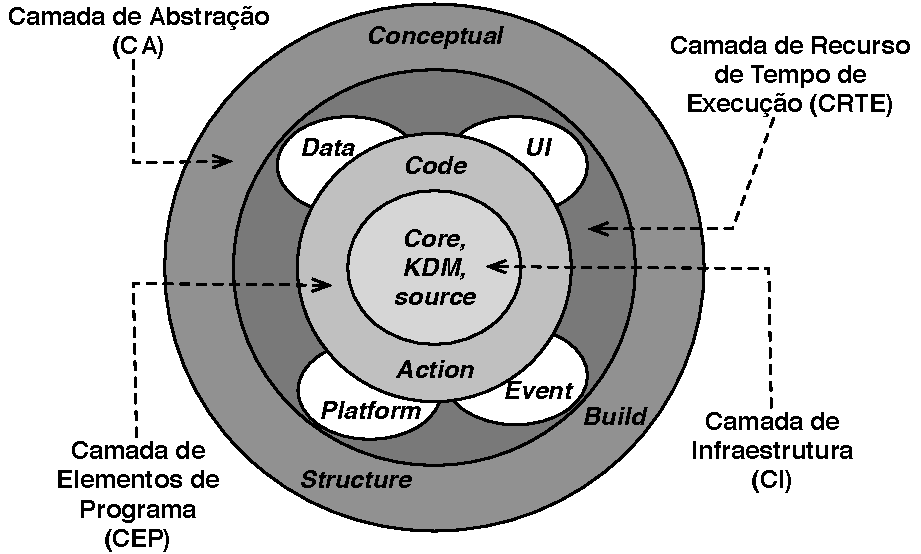
\includegraphics[scale=0.67]{images/kdm_layers.pdf}
 \fadaptada{KDM:specification}
\end{figure}
%
A camada CI contém três pacotes, são eles: (\textit{i}) \texttt{Core}, (\textit{ii}) \texttt{\aspas{kdm}} e (\textit{iii}) \texttt{Source}. Os dois primeiros pacotes, \texttt{Core} e \texttt{\aspas{kdm}}, representam a infraestrutura básica para outros pacotes do KDM e definem metaclasses e relacionamentos básicos. O pacote \texttt{Source} define o \texttt{Inventory Model}, o qual representa artefatos de software e mantêm a rastreabilidade entre eles. 

A camada CEP possui dois pacotes: (\textit{i}) \texttt{Code} e (\textit{ii}) \texttt{Action}. Esses pacotes coletivamente definem o \texttt{Code Model} que contém metaclasses para representar artefatos em nível de implementação. O pacote \texttt{Code} contém um conjunto de metaclasses para representar a estrutura de um determinado programa e seus relacionamentos, enquanto que o pacote \texttt{Action} possui metaclasses para descrever o comportamento e o fluxo de dados de um programa.

A camada CRTE contém quatro pacotes: (\textit{i}) \texttt{Data}, (\textit{ii}) \texttt{Platform}, (\textit{iii}) \texttt{Event} e (\textit{iv}) \texttt{UI}. Coletivamente tais pacotes representam a estrutura e comportamento de recursos de tempo de execução do sistema. Tais pacotes são diretamente instanciados por meio da definição de recursos, abstração do \texttt{Code Model}, ou são manualmente instanciado pelo engenheiro de modernização. A rastreabilidade entre os elementos abstraídos e os elementos físicos (por exemplo, código-fonte) é mantida pelo meta-atributo denominado \texttt{implementation}. Finalmente, a camada CA contém três pacotes: (\textit{i}) \texttt{Conceptual}, (\textit{ii}) \texttt{Structure} e (\textit{iii}) \texttt{Build}. Esses pacotes possuem metaclasses para representar o maior nível de abstração de um sistema, por exemplo, a estrutura do sistema, regras de negócios, documentações do sistema, etc.

Uma característica importante de ser observada e ressaltada é que todas as camadas do KDM interagem, significando que todas as camadas são conectadas de alguma forma\footnote{Essa conectividade entre os elementos de cada camada são mantidos por um conjunto de meta-atributo, por exemplo, o meta-atributo \texttt{implementation}.}, como consequência se uma mudança/refatoração é realizada em uma camada especifica, a mudança/refatoração deve ser propagada para outras camadas com o intuito de manter todas as camadas sincronizadas e consistentes preservando assim a estrutura estática do KDM e o comportamento do código representado em KDM. Nas próximas seções são apresentados os principais pacotes do metamodelo KDM que compõem o contexto para o desenvolvimento deste trabalho.

\subsection{Pacote Code}\label{subsection:codePackage}

O pacote $\mathtt{Code}$ define um conjunto de metaclasses cujo propósito é representar unidades de programa em nível de implementação e as suas associações. O pacote também inclui metaclasses que representam elementos de programa comuns suportados por várias linguagens de programação, como tipo de dados, classes, procedimentos, macros, protótipos e \textit{templates}.


Em uma determinada instância do KDM, cada elemento do pacote~$\mathtt{code}$ representa alguma construção em uma linguagem de programação, determinada pela linguagem de programação utilizada no sistema. Na Figura~\ref{fig:CodeModel} um trecho do~$\mathtt{CodeModel}$\footnote{O diagrama de classes do $\mathtt{CodeModel}$ mostrado aqui só representa o conjunto de metaclasses e os seus respectivos relacionamentos lógicos, para informações completas, verifique a especificação do KDM~\cite{KDM:specification}.} é retratado.

%In a given KDM instance, each instance of the code metamodel element represents some programming language construct, determined by the programming language of the existing software system. Each instance of a code metamodel element corresponds to a certain region of the source code in one of the artifacts of the existing software system. Figure~\ref{fig:CodeModel} the \texttt{CodeModel}\footnote{The \texttt{CodeModel} class diagram presented herein shows just a set of the metaclasses and their logical relationship, for complete information please see the KDM specification} is depicted, it represents parts of the KDM infrastructure. 

\begin{figure}[!ht]
	\centering
	% Requires \usepackage{graphicx}
	\caption{Diagrama de classes - $\mathtt{CodeModel}$}
	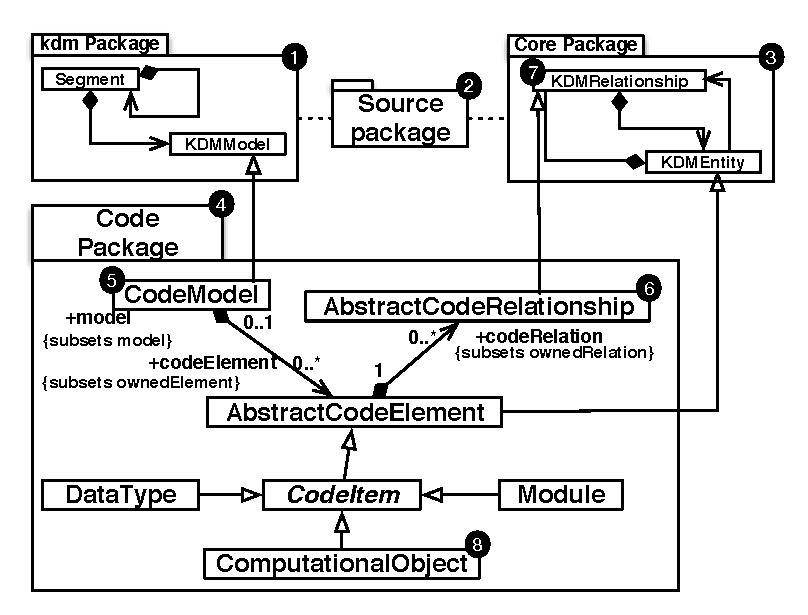
\includegraphics[scale=0.67]{images/codeModel}
	\label{fig:CodeModel}
	\fadaptada{KDM:specification}
\end{figure}

A metaclasse \texttt{CodeModel} representa um contêiner para outras instâncias de elementos do tipo~$\mathtt{Code}$. O pacote $\mathtt{Code}$ \ding{205} depende dos outros pacotes $\mathtt{kdm}$ \ding{202}, $\mathtt{Source}$ \ding{203} e $\mathtt{Core}$ \ding{204}. A metaclasse $\mathtt{CodeModel}$ \ding{206} é um modelo que possui coleções de fatos sobre o sistema de software, correspondentes ao domínio $\mathtt{Code}$. Ela possui uma associação  $\mathtt{codeElement:AbstractCodeElement[0..*]}$ permitindo a adição de novos elementos de código, por exemplo, métodos, atributos, etc. A metaclasse  $\mathtt{AbstractCodeRelationship}$ \ding{207} representa qualquer relacionamento determinado por em uma linguagem de programação. Por sua vez, a metaclasse $\mathtt{ComputationalObject}$ representa os elementos determinados pela linguagem de programação, que descreve certos objetos computacionais em tempo de execução, por exemplo, métodos e variáveis.

%This metamodel element is a container for other \texttt{code} element instances. As can be observed in Figure~\ref{fig:CodeModel} the \texttt{Code} package \ding{205} depends on the \texttt{kdm} \ding{202}, \texttt{Source} \ding{203}, and \texttt{Core} \ding{204} packages. The meta-class \texttt{CodeModel} \ding{206} is the specific KDM model that owns collections of facts about the existing software system such that these facts correspond to the \texttt{Code} domain, its superclass is \texttt{KDMModel}. It has as association \texttt{codeElement:AbstractCodeElement[0..*]} meaning that one shall arrange code elements (e.g., methods, fields, etc) into one or more code models. The \texttt{AbstractCodeRelationship} \ding{207} is an abstract meta-class representing any relationship determined by a programming language, it is also used to constrain the subclasses of \texttt{KDMRelationship} (see Figure~\ref{fig:CodeModel} \ding{208}) in the \texttt{Code} model. The meta-class \texttt{ComputationalObject} represents the named elements determined by the programming language, which describe certain computational objects at the runtime, for example, methods, and variables.

O pacote~$\mathtt{Code}$ consiste em um total de 24 metaclasses; tais metaclasses são um arranjo de abstrações para representar toda, ou a grande maioria, da estrutura estática de um terminado código-fonte dado um linguagem de programação, seja ela procedural ou orientada a objetos~\cite{KDM:specification}. Na Tabela~\ref{tab:meta_classes_pacoteCODE} algumas metaclasses são apresentadas. Como pode ser observado algumas metaclasses podem ser diretamente elucidadas e mapeadas, como por exemplo, \aspas{classes} e \aspas{interfaces} construções facilmente encontradas em linguagens orientadas a objetos podem ser facilmente mapeada para as metaclasses denominada $\mathtt{ClassUnit}$ e $\mathtt{InterfaceUnit}$, respectivamente. Um mapeamento mais completo entre elementos estruturais e metaclasses do KDM pode ser identificado em~\citeonline{bruno_marinho_dissertacao} e no Capítulo~\ref{chapter:catalogo_refactoring_KDM}. Uma representação dessas metaclasses, bem como seus relacionamentos são apresentados em diagrama de classe na Figura~\ref{fig:classUnit_e_InterfaceUnit}.

\begin{figure}[!ht]
	\centering
	\caption{Diagrama de classes elucidando as metaclasses \texttt{ClassUnit} e \texttt{InterfaceUnit}}
	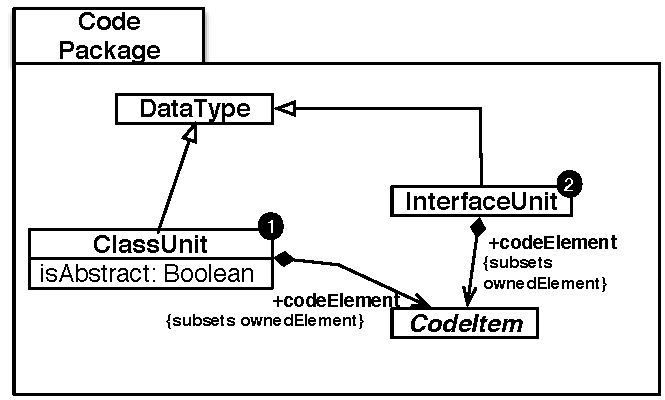
\includegraphics[scale=0.67]{images/ClassUnit_InterfaceUnit}
	\label{fig:classUnit_e_InterfaceUnit}
	\fadaptada{KDM:specification}
\end{figure}

%The whole \texttt{Code} package consists of $24$ metaclasses\footnote{Note that not all the meta-class are shown in Figure~\ref{fig:CodeModel}} and contains all the abstract elements for modeling the static structure of the source code. In Table~\ref{tab:mappingCodeToKDM} is depicted some of them. This table identifies KDM metaclasses possessing similar characteristics to the static structure of the source code. Some metaclasses can be direct mapped, such as class from object-oriented language, which can be easily mapped to the \texttt{ClassUnit} meta-class from KDM. For instance, the meta-class \texttt{Package} is a subtype for \texttt{Module} that logical collections of program elements, as directly supported by some programming languages, such as Java. 

\begin{table}[h]
\centering
\caption{Metaclasses para modelagem de estruturas estáticas do código-fonte.}
\label{tab:meta_classes_pacoteCODE}
\begin{tabular}{|l|l|}
\hline
Elemento do Código-Fonte & metaclasses do KDM \\ \hline
\multicolumn{1}{|c|}{Classe}                   & \multicolumn{1}{|c|}{\texttt{ClassUnit}}           \\ \hline
\multicolumn{1}{|c|}{Interface}                & \multicolumn{1}{|c|}{\texttt{InterfaceUnit}}       \\ \hline
\multicolumn{1}{|c|}{Método}                   & \multicolumn{1}{|c|}{\texttt{MethodUnit}}          \\ \hline
\multicolumn{1}{|c|}{Atributo}                 & \multicolumn{1}{|c|}{\texttt{StorableUnit}}        \\ \hline
\multicolumn{1}{|c|}{Variável Local}           & \multicolumn{1}{|c|}{\texttt{MemberUnit}}          \\ \hline
\multicolumn{1}{|c|}{Parâmetro}                & \multicolumn{1}{|c|}{\texttt{ParameterUnit}}       \\ \hline
\multicolumn{1}{|c|}{Associação}               & \multicolumn{1}{|c|}{\texttt{KDMRelationShip}}     \\ \hline
\end{tabular}
\end{table}

%\begin{table}[!h]
	%\caption{metaclasses para modelagem de estruturas estáticas do código fonte}
%	\label{tab:mappingCodeToKDM}
%	\centering
%	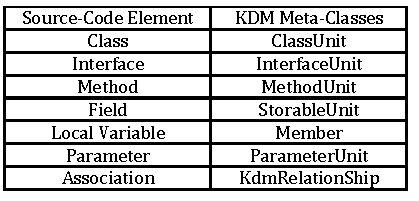
\includegraphics[scale=1]{images/tabela_comparativo_KDM_code_com_source_code}
%\end{table}

$\mathtt{ClassUnit}$ e $\mathtt{InterfaceUnit}$ representam \aspas{classes} e \aspas{interfaces} que são definidas por usuários de linguagens orientadas a objeto. Ambas metaclasses possuem caracteristicas e relacionamentos similares, como observado na Figura~\ref{fig:classUnit_e_InterfaceUnit} \ding{202} e \ding{203}. Uma das diferenças que pode ser destacada é que a metaclasse ~$\mathtt{ClassUnit}$ contém um meta-atributo~$\mathtt{isAbstract:Boolean}$, o qual é utilizado para especificar se uma classe é ou não abstrata. $\mathtt{ClassUnit}$ e $\mathtt{InterfaceUnit}$ podem conter um coleção de elementos que seja do tipo ~$\mathtt{CodeItem}$, por exemplo,~$\mathtt{StorableUnit}$ ou ~$\mathtt{MethodUnit}$. Além disso, tais metaclasses  possuem uma meta-associação denominada ~$\mathtt{codeElement:CodeItem[0..*]}$ que é utilizada para agrupar todos os membros da classe, por exemplo, construtores, métodos, atributos, etc. Na Figura~\ref{fig:StorableUnit_MethodUnit} é apresentado os meta-atributos e metarelacionamentos das metaclasses \texttt{StorableUnit} \ding{204}, \texttt{MethodUnit} \ding{205}, \texttt{ParameterUnit} \ding{207} e \texttt{MemberUnit} \ding{206}.

\begin{figure}[!ht]
	\centering
	% Requires \usepackage{graphicx}
	\caption{Diagrama de classes elucidando as metaclasses \texttt{StorableUnit}, \texttt{MethodUnit}, \texttt{ParameterUnit} e \texttt{MemberUnit}}
	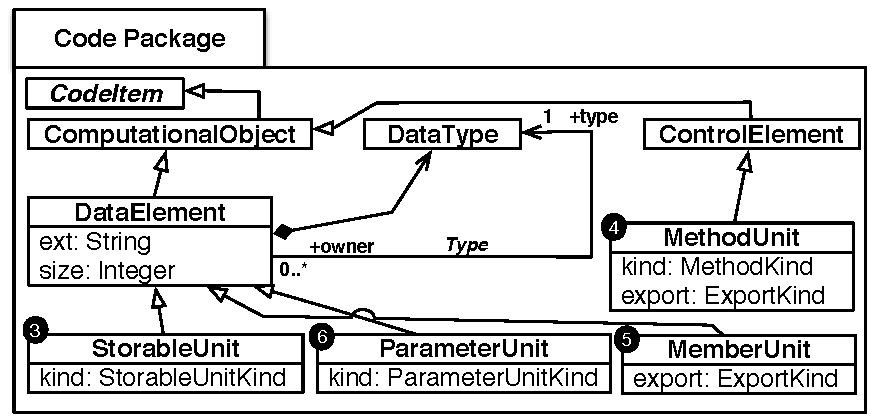
\includegraphics[scale=0.67]{images/StorableUnit_MethodUnit2}
	\label{fig:StorableUnit_MethodUnit}
	\fadaptada{KDM:specification}
\end{figure}


%As stated before, the meta-class \texttt{ClassUnit} represents user-defined classes in object-oriented languages. A class datatype is a named datatype that represents a class: an ordered collection of named elements, each of which can be another \texttt{CodeItem}, such as a \texttt{StorableUnit} or a \texttt{MethodUnit}. The meta-class \texttt{ClassUnit} contains a meta-attribute \texttt{isAbstract:Boolean} used to specify if the class is abstract or not. \texttt{ClassUnit} also has an meta-association named \texttt{codeElement:CodeItem[0..*]} that is used to group all class's members, e.g., fields, constructor, methods, etc. 

%Similarmente, a metaclasse~$\mathtt{InterfaceUnit}$ representa o conceito comum a várias linguagens de programação. Ela é uma subclasse de~$\mathtt{DataType}$, assim como~$\mathtt{ClassUnit}$.~$\mathtt{InterfaceUnit}$ também possui uma meta associação chamada~$\mathtt{codeElement:CodeItem[0..*]}$ que representa tipos de dados tal como~$\mathtt{MethodUnit}$.

%Similarly, the meta-class \texttt{InterfaceUnit} represents the interface concept common to various programming languages. It is also a subclass of \texttt{Datatype} as \texttt{ClassUnit}. \texttt{InterfaceUnit} also has an meta-association named \texttt{codeElement:CodeItem[0..*]} that represent data types as well as \texttt{MethodUnits}.

$\mathtt{StorableUnit}$ representa um atributo em um sistema de software - um objeto computacional para que diferentes valores do mesmo tipo de dados possa ser associado em vezes diferentes. Ele é usado para representar as variáveis globais e locais. Ele contém uma meta atributo~$\mathtt{String}$ usado para definir o nome das variáveis.~$\mathtt{StorableUnit}$ também tem a associação~$\mathtt{type:DataType[1]}$, a qual é herdada da metaclasse~$\mathtt{DataElement}$, e é utilizado para especificar o tipo da variável (\textit{int, char, boolean, numeric}, etc). Ele também tem uma enumeração ~$\mathtt{kind:StorableUnit}$, que descreve várias propriedades comuns de um ~$\mathtt{StorableUnit}$ relacionado com o seu ciclo de vida, por exemplo, sua visibilidade (\textit{private, public, protected}, etc).

%\texttt{StorableUnit} represents a variable of existing software system - a computational object to which different values of the same datatype can be associated at different times. It is used to represent both global and local variables. It contains a meta-attribute \texttt{name:String} used to set the name of the variables. \texttt{StorableUnit} also has the association \texttt{type:Datatype[1]} used to specify the variable's type. It also has a enumeration \texttt{kind:StorableKind}, it describes several common properties of a \texttt{StorableUnit} related to their life-cycle, visibility, and memory type. 

~$\mathtt{MethodUnit}$ como o próprio nome sugere representa métodos que são identificados em ~$\mathtt{ClassUnit}$ ou~$\mathtt{InterfaceUnit}$. Ele também é usado para representar construtores e destrutores. Possui como meta-atributos~$\mathtt{name:String}$,~$\mathtt{kind:MethodKind}$ e ~$\mathtt{export:ExportKind}$. O primeiro é usado para descrever o nome de um método. O segundo meta-atributo é uma enumeração que define especificações adicionais do tipo de método, ou seja, é possível especificar se a instância do método é um construtor, destrutor, ou um método normal. O último representa a visibilidade do método (\textit{private, public, protected}, etc).

%\texttt{MethodUnit} represents member functions owned by either \texttt{ClassUnit} or \texttt{InterfaceUnit}. It is also used to represent user-defined operators, constructors, and destructors. It owns as meta-attributes \texttt{name:String}, \texttt{kind:MethodKind}, and \texttt{export: ExportKind}. The fist one is used to describe to name of a method. The second meta-attribute is an enumeration that defines additional specification of the kind of method, i.e., it is possible to specify if the method's instance is a constructor, destructor, abstract, etc. The last one represents the visibility of the method, i.e., \texttt{public}, \texttt{private}, \texttt{protected}.

A fim de entender como o KDM é utilizado para representar estruturas um determinado programa, no Código-fonte~\ref{lst:example_kdm_instance} é mostrado um exemplo simplificado escrito em Java. O correspondente KDM, embora simplificado, é apresentado na Figura~\ref{fig:kdm_instance_Java}. Por questões de simplicidade e para facilitar o entendimento, essa figura ilustra a instância do KDM em forma de um diagrama de objetos; é possível notar que este diagrama representa o código-fonte como uma árvore, na qual cada nó representa uma metaclasses do KDM. Como pode ser visto na Figura~\ref{fig:kdm_instance_Java}, a metaclasse raiz é ~$\mathtt{Segment}$, que é um recipiente para um conjunto significativo de fatos sobre um sistema de software existente. Cada~$\mathtt{Segment}$ pode incluir uma ou mais instâncias de modelos do KDM, como~$\mathtt{CodeModel}$ e~$\mathtt{StructureModel}$.

%In order to fully understand how KDM is used to represent the source code of a specific program, in Listing~\ref{lst:example_kdm_instance} is shown a simplified example in Java. The corresponding, though simplified KDM instance is depicted in Figure~\ref{fig:kdm_instance_Java}. It illustrates a KDM instance as a UML object diagram for the sake of simplicity, note that this diagram represents the source code as a tree of nodes containing some KDM's metaclasses. As can be seen in Figure~\ref{fig:kdm_instance_Java} the root meta-class is \texttt{Segment}, which is a container for a meaningful set of facts about an existing software system. Each \texttt{Segment} may include one or more KDM model instances, such as \texttt{CodeModel} and \texttt{StructureModel}. As stated earlier, the \texttt{CodeModel} is the specific KDM container for other \texttt{code} element instances (see Figure~\ref{fig:CodeModel}). 

Analisando tanto o Código-fonte~\ref{lst:example_kdm_instance} quanto a Figura~\ref{fig:kdm_instance_Java} é evidente que cada estrutura estática do código-fonte tem uma metaclasse específica em KDM para representá-la. Por exemplo, a declaração \textit{package} \textit{model} na Linha 1 do Código-fonte~\ref{lst:example_kdm_instance} \ding{202} é representada em KDM pela metaclasse ~$\mathtt{package}$, como visto na Figura~\ref{fig:kdm_instance_Java} \ding{202}. Posteriormente, como apresentado no Código-fonte~\ref{lst:example_kdm_instance} \ding {203} uma classe~$\mathtt{Car}$ é declarada. Essa classe herda caracteristicas da classe~$\mathtt{Vehicle}$, no Java isso é feito por meio da palavra-chave~$\mathtt{extends}$ seguido do nome de uma classe, conforme por ser observado no Código-fonte~\ref{lst:example_kdm_instance} \ding{204} e \ding{205}. A metaclasse~$\mathtt{Extends}$ representa o conceito de herança em KDM. Como mostrado na Figura~\ref{fig:kdm_instance_Java} \ding {204} a metaclasse~$\mathtt{Extends}$ possui duas associações,~$\mathtt{to}$ e~$\mathtt{from}$, o primeiro representa a classe pai (\textit{super class}), e o último a classe filha(\textit{sub-class}). Neste contexto, a classe~$\mathtt{Car}$ e classe pai de~$\mathtt{Vehicle}$, como mostrado na Figura~\ref{fig:kdm_instance_Java} \ding{205}. Finalmente, o atributo~$\mathtt{name}$ e o método~$\mathtt{getName()}$ (ver Código-fonte~\ref{lst:example_kdm_instance} \ding {206} e \ding {207}, respectivamente) são mapeados para os correspondentes elementos do KDM,~$\mathtt{StorableUnit}$ e~$\mathtt{MethodUnit}$ (ver Figura ~\ref{fig:kdm_instance_Java} \ding {206} e \ding {207}). 

%Analyzing both the Listing~\ref{lst:example_kdm_instance} and the Figure~\ref{fig:kdm_instance_Java} it is evident that each static structure of the source code has a meta-class in KDM to represent it. For instance, the package model in Line 1 of Listing~\ref{lst:example_kdm_instance} \ding{202} is represented in KDM by the meta-class named \texttt{Package}, see Figure~\ref{fig:kdm_instance_Java} \ding{202}. In addition, the class \texttt{Car} is declared, see Listing~\ref{lst:example_kdm_instance} \ding{203}. It also inherit from class \texttt{Vehicle}, in the Java this is accomplished by using the keyword \texttt{extends} following of a class, see Listing~\ref{lst:example_kdm_instance}  \ding{204} and \ding{205}. The meta-class \texttt{Extends} represents inheritance in KDM models. As shown in Figure~\ref{fig:kdm_instance_Java} \ding{204} the meta-class \texttt{Extends} has two association, \texttt{to} and \texttt{from}, the former represents the parent class (super class), and the latter represents the child class (sub-class). In this context, the child is the class \texttt{Car} and the parent class is \texttt{Vehicle}, which is depicted in Figure~\ref{fig:kdm_instance_Java} \ding{205}. Finally, the variable \texttt{name}, and the method \texttt{getName()} (see Listing~\ref{lst:example_kdm_instance} \ding{206}, and \ding{207}) are mapped to corresponding instances of the KDM elements, \texttt{StorableUnit}, and \texttt{MethodUnit} (see Figure~\ref{fig:kdm_instance_Java} \ding{206}, and \ding{207}). 


\noindent\begin{minipage}{.53\textwidth}
	\begin{codigo}[caption={[Parte de código Java para ilustrar como o KDM é usado para representar o código fonte.] Simples código em java.},escapeinside={(*@}{@*)}, basicstyle=\footnotesize, label={lst:example_kdm_instance}]{Name}
	(*@\ding{202}@*) package model;
	(*@\ding{203}@*) public class Car (*@\ding{204}@*) extends  
	(*@\ding{205}@*) Vehicle{
	(*@\ding{229}@*)(*@\ding{206}@*) private String name;
	(*@\ding{229}@*)(*@\ding{207}@*) public String getName(){
	(*@\ldots @*)
	}
	}
	\end{codigo}
\end{minipage}\hfill
\begin{minipage}{.45\textwidth}
	\centering
	% Requires \usepackage{graphicx}
	\captionof{figure}{Instância KDM correspondente ao Código-fonte~\ref{lst:example_kdm_instance}}
	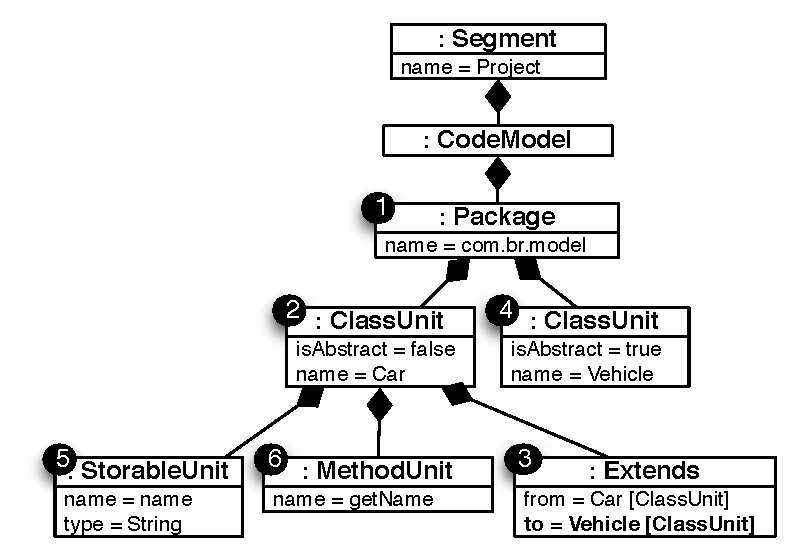
\includegraphics[scale=0.6]{images/kdm_instance_java_correspoding_2_with_extends}
	\fautor
	\label{fig:kdm_instance_Java}
\end{minipage}


Apenas metaclasses utilizadas para representar estruturas e construções estáticas foram apresentadas. No entanto, o KDM contém um pacote que permite a representação de construções dinâmicas, em outras palavras, o pacote \textit{Action} contém metaclasses cuja finalidade é permitir e representar comportamento em nível de execução. Na seção a seguir mais informações sobre esse pacote é apresentado.

\subsection{Pacote Action}\label{sec:actionPackage}

O pacote~$\mathtt{Action}$ define um conjunto de metaclasses, cujo propósito é o de representar descrições de comportamento em nível de implementação estabelecido por linguagens de programação, por exemplo, declarações, operadores, condições e as suas associações. A Figura ~\ref{fig:actionModel} \ding {202} mostra o pacote~$\mathtt{Action}$ e algumas de suas metaclasses. Como pode ser observado, este pacote estende o pacote~$\mathtt{Code}$ (ver a Figura~\ref {fig:actionModel} \ding {208}).

%The \texttt{Action} package defines a set of metaclasses whose purpose is to represent implementation-level behavior descriptions determined by programming languages, for example statements, operators, conditions, features, as well as their associations, for example control and data flow. The Figure~\ref{fig:actionModel} \ding{202} shows the\texttt{Action} package and some of its metaclasses. As can be observed it extends the KDM \texttt{Code} package (see Figure~\ref{fig:actionModel} \ding{208}). 

\begin{figure}[!ht]
	\centering
	% Requires \usepackage{graphicx}
	\caption{Diagrama de classes ilustrando o pacote~$\mathtt{Action}$.}
	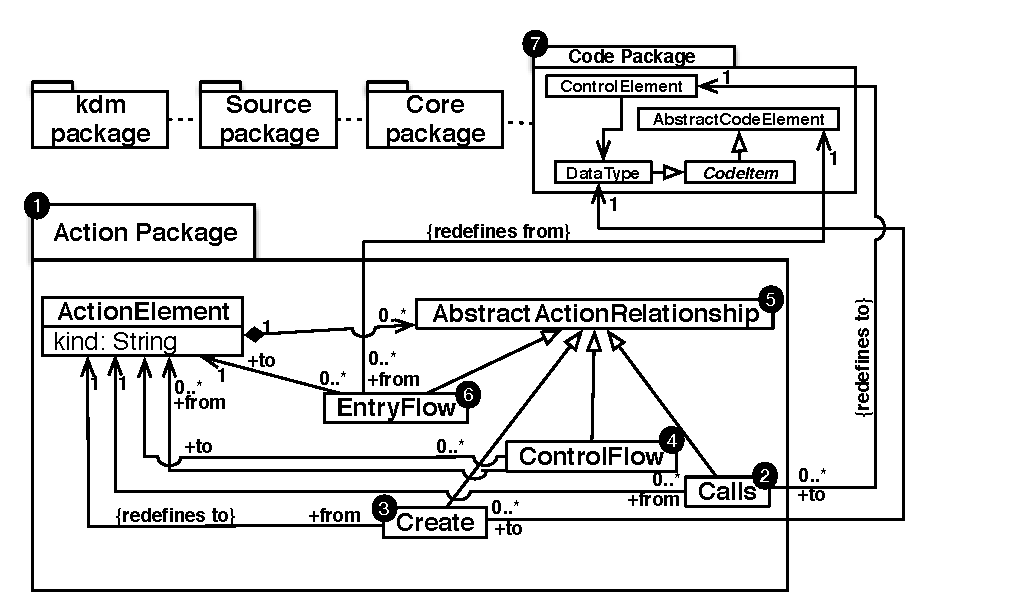
\includegraphics[scale=0.67]{images/ActionModel_Class_Diagram}
	\label{fig:actionModel}
	\fadaptada{KDM:specification}
\end{figure}

O pacote~$\mathtt{Action}$ é composto por 11 diagramas de classe, ele também depende dos pacotes~$\mathtt{Core}$, ~$\mathtt{kdm}$ e ~$\mathtt{Source}$, e  principalmente do pacote~$\mathtt{Code}$. No entanto, o pacote~$\mathtt{Action}$ segue o padrão uniforme para os modelos KDM e estende o KDM com metaclasses específicas relacionadas com o comportamento do nível de implementação. O pacote~$\mathtt{Action}$ se desvia de um padrão uniforme para os modelos KDM porque ele não define um modelo KDM separado, mas estende o pacote~$\mathtt{Code}$.  Por isso, cada metaclasse do pacote ~$\mathtt{Action}$ é uma subclasse de~$\mathtt{AbstractCodeElement}$, conforme destacado na Figura~\ref{fig:actionModel}. O pacote~$\mathtt{Action}$ define a maioria das metaclasses que tem como objetivo representar comportamentos para as construções estáticas definidas no pacote~$\mathtt{Code}$. Assim, ambos pacotes constituem a CEP, como mostrado na Figura~\ref{fig:kdm_layer}.

%The \texttt{Action} package consists of 11 class diagrams, it also depends on the \texttt{Core}, \texttt{kdm}, \texttt{Source}, and mainly \texttt{Code}. However, the \texttt{Action} package follows the uniform pattern for KDM models and extends the KDM with specific metaclasses related to implementation-level behavior. The \texttt{Action} package deviates from a uniform pattern for KDM models because it does not define a separate KDM model, but rather extends the \texttt{Code}, which is presented in Section~\ref{codePackage}. Therefore each \texttt{Action} metaclasses is a subclass of \texttt{AbstractCodeElement}, as highlighted in Figure~\ref{fig:actionModel}. \texttt{Action} package defines most of the relationship types to the \texttt{Code} model. Together, \texttt{Action}, and \texttt{Code} packages constitute the Program Elements Layer of KDM as depicted in Figure~\ref{fig:all_kdm_layers}. 

A metaclasse~$\mathtt{AbstractionActionRelationship}$ apresentada na Figura~\ref{fig:actionModel} \ding{206} é a metaclasse pai usada para representar várias relações que se originam a partir de um~$\mathtt{ActionElement}$. Além disso, essa metaclasse~$\mathtt{AbstractionActionRelationship}$ possui metaclasses específicas; algumas delas estão representadas na Figura~\ref{fig:actionModel}, por exemplo, as metaclasses~$\mathtt{Calls}$ \ding {203},~$\mathtt{Creates}$ \ding {204},~$\mathtt{ControlFlow}$ \ding {205} e~$\mathtt{EntryFlow}$ \ding{207}.

%The meta-class \texttt{AbstractActionRelationship} presented in Figure~\ref{fig:actionModel} \ding{206} is the parent class used to represent various KDM relationships that originate from an \texttt{ActionElement}. The meta-class \texttt{AbstractActionRelationship} owns specific metaclasses. Some of them are depicted in Figure~\ref{fig:actionModel}, for example, the metaclasses \texttt{Calls} \ding{203}, \texttt{Create} \ding{204}, \texttt{ControlFlow} \ding{205}, and \texttt{EntryFlow} \ding{207}.

O relacionamento~$\mathtt{Calls}$ corresponde a uma chamada para um procedimento, um método estático, um método não-estático de uma instância particular de um objeto, um método virtual, ou um elemento de interface.~$\mathtt{Calls}$ possui duas associações, são elas: ~$\mathtt{ActionElement[1]}$ e ~$\mathtt{ControlElement[1]}$. O primeiro representa o elemento de ação a partir do qual a relação chamada origina, a segunda associação representa o elemento alvo.

%\texttt{Calls} relationship corresponds to ``invoke'' operation on a procedure type. It can represent a call to a procedure, a static method, a non-static method of a particular object instance, a virtual method, or an interface element. \texttt{Calls} has two associations, they are: \texttt{from:ActionElement[1]} and \texttt{to:ControlElement[1]}. The first one represents the action element from which the call relation originates. The second association represents the target \texttt{ControlElement}.

A metaclasse~$\mathtt{Creates}$ representa uma associação entre um elemento de ação que \aspas{cria} uma nova instância de um determinado elemento de dados. Por exemplo, em Java essa metaclasse corresponde a palavra-chave \textit{new} utilizada para instânciar um novo objeto. $\mathtt{Creates}$ também possui duas associações:~$\mathtt{ActionElement[1]}$ e~$\mathtt{DataType[1]}$. Similar a metaclasse~$\mathtt{Calls}$, a primeira associação representa o elemento que possui o relacionamento e a segunda representa o elemento de dados (objeto) que é instanciado pelo~$\mathtt{ActionElement}$.

%The meta-class \texttt{Create} represents an association between an action element that ``creates'' a new instance of a certain data element to the corresponding datatype according to the semantics of the programming language of the existing software system. It also has association, \texttt{from:ActionElement[1]} and \texttt{to:Datatype[1]}. Similarly, to the meta-class \texttt{Calls}, the first association represents the element that owns the \texttt{Creates} relationship. The second one illustrates the \texttt{DataElement} that is instantiated by the \texttt{ActionElement}. 

O~$\mathtt{ControlFlow}$ é um elemento de modelagem genérica que representa relação de fluxo de controle entre dois~$\mathtt{ActionElements}$. Além disso, é uma submetaclasse com elementos de modelagem mais específicas. O~$\mathtt{EntryFlow}$ é um elemento de modelagem que representa um fluxo inicial de controle em um elemento KDM. O relacionamento~$\mathtt{EntryFlow}$ é usado de uma maneira uniforme para descrever os pontos de entrada para outros elementos de código KDM.

%The \texttt{ControlFlow} is a generic modeling element that represents control flow relation between two \texttt{ActionElements}. It is further subclassed with more specific modeling elements. The \texttt{EntryFlow} is a modeling element that represents an initial flow of control into a KDM element. The \texttt{EntryFlow} relationship is used in a uniform way for describing entry points to other KDM code elements. 

A fim de compreender como o pacote~$\mathtt{Action}$ é usado no KDM, no Código-fonte~\ref{lst:example_kdm_instance_2} é mostrado um simples método implementado em Java. Neste método é criada uma instância de~$\mathtt{Car}$ e seu método de acesso é invocado. Uma possível correspondente instância do KDM simplificada é apresentada na Figura~\ref{fig:kdm_instance_Java_action}. Nota-se que, o diamante em destaque na cor cinza e anexado com três pontos (\ldots) ilustra que outras metaclasses não são mostrados com o intuito de simplificar a figura.

%In order to comprehend  how the \texttt{Action} package is used in KDM, in Listing~\ref{lst:example_kdm_instance_2} shows a simple method implemented in Java. In this method is created an instance of \texttt{Car} and an accessor method of it is called, ie., the \texttt{getName()}. The corresponding simplified KDM instance is depicted in Figure~\ref{fig:kdm_instance_Java_action}. Please note that, the diamond highlighted in grey and attached with three dots (\ldots) illustrates that other metaclasses are not shown in order to simplify the figure.  

\noindent\begin{minipage}{.43\textwidth}
	\begin{codigo}[caption={[Pedaço de código Java para ilustrar como o pacote~$\mathtt{Action}$ funciona.] Método \texttt{e1} ilustrando como o Pacote \texttt{Action} funciona.}, escapeinside={(*@}{@*)}, basicstyle=\footnotesize, label={lst:example_kdm_instance_2}]{Name}
	(*@\ldots @*)
	public void e1 (*@\ding{202}@*)(){
	Car myCar (*@\ding{203}@*) = new Car() (*@\ding{204}@*);
	(*@\ding{229}@*)myCar.getName() (*@\ding{205}@*);
	}
	(*@\ldots @*)
	\end{codigo}
\end{minipage}\hfill
\begin{minipage}{.65\textwidth}
	\centering
	\captionof{figure}{Instância KDM correspondente ao Código-fonte~\ref{lst:example_kdm_instance_2}}
	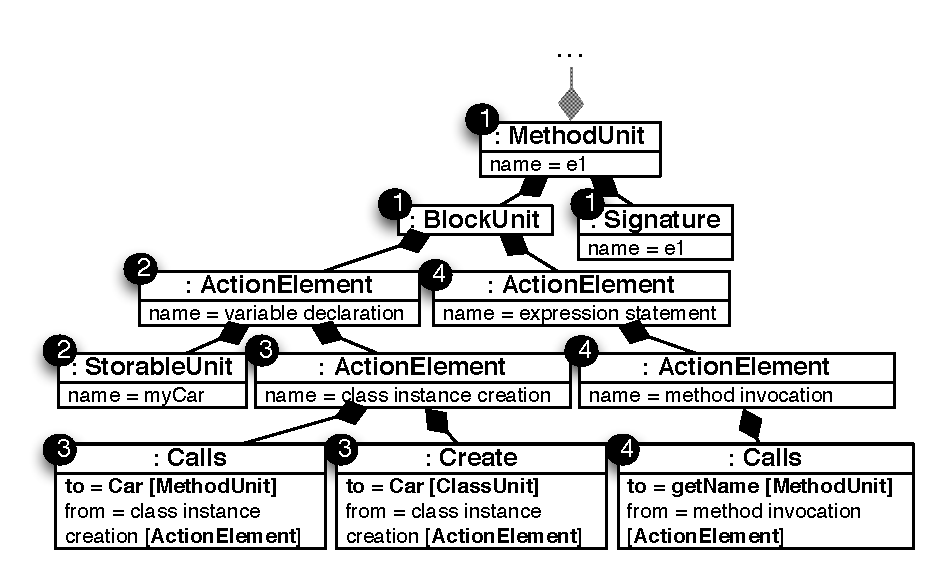
\includegraphics[scale=0.6]{images/actionInstanceKDM_2}
	\fautor
	\label{fig:kdm_instance_Java_action}
\end{minipage}

As três primeiras metaclasses mostradas nesta hierarquia são~$\mathtt{MethodUnit}$,~$\mathtt{BlockUnit}$ e~$\mathtt{Signature}$ conforme destacado na  Figura~\ref{fig:kdm_instance_Java_action} \ding{202}. Essas três metaclasses basicamente representam uma declaração e a assinatura de um determinado método, no caso \texttt{e1()}. Mais especificamente, a metaclasse~$\mathtt{MethodUnit}$ é usada para representar o método~$\mathtt{e1()}$ como mostrado tanto no Código-fonte~\ref{lst:example_kdm_instance_2} \ding{202} e na Figura~\ref{fig:kdm_instance_Java_action} \ding{202}.~$\mathtt{BlockUnit}$ representa blocos lógicos e físicos relacionados de~$\mathtt{ActionElement}$, ou seja, o escopo do método representado por \{...\}. Por sua vez,~$\mathtt{Signature}$ representa a assinatura do método, isto é, essa metaclasse representa além do nome do método todos os parâmetros, o retorno do método, exceções, etc.	

%The first three metaclasses shown in this hierarchy are the \texttt{MethodUnit}, \texttt{BlockUnit}, and \texttt{Signature} (see Figure~\ref{fig:kdm_instance_Java_action} \ding{202}). These metaclasses are used to represent a simple method declaration. More specifically, the meta-class \texttt{MethodUnit} is used to represent the method \texttt{e1} as shown in both Listing~\ref{lst:example_kdm_instance_2} \ding{202} and Figure~\ref{fig:kdm_instance_Java_action} \ding{202}. \texttt{BlockUnit} represents logically and physically related blocks of \texttt{ActionElement}, i.e., the area between the braces, \texttt{\{\ldots\}}. In turn, \texttt{Signature} represents the concept of a method signature, i.e., it also can be used to represent the name of the method, all the parameters, the return of the method, etc.

Na Linha 12 do Código-fonte~\ref{lst:example_kdm_instance_2} \ding{203} uma variável chamada~$\mathtt{myCar}$ é declarada. As metaclasses que representam esta declaração podem ser visualizadas na Figura~\ref{fig:kdm_instance_Java_action} \ding{203}. A metaclasse~$\mathtt{ActionElement}$ representa o significado das operações, por exemplo, um declaração da variável. A metaclasse~$\mathtt{StorableUnit}$ representa a própria variável, \texttt{myCar}. Ainda na Linha 10 \ding{204} a instância da classe~$\mathtt{Car}$ é criada usando a palavra-chave~$\mathtt{new}$. Nota-se que na Figura~\ref{fig:kdm_instance_Java_action} \ding{204} três metaclasses são utilizadas para representar o operador~$\mathtt{new}$. Primeiramente, a metaclasse~$\mathtt{ActionElement}$ é usada para ilustrar o significado da operação, neste caso, a instância da classe \texttt{Car}. A metaclasse~$\mathtt{Calls}$ é usada para ilustrar a instanciação de um objeto, neste caso, o objeto~$\mathtt{Car}$. Adicionalmente, a metaclasse \texttt{Calls} posssui duas ~$\mathtt{to}$ e~$\mathtt{from}$, as quais representam a chamada para o construtor de~$\mathtt{Car}$ e representa o alvo~$\mathtt{ActionElement}$, respectivamente. Em seguida, a metaclasse~$\mathtt{Creates}$ representa a nova instância de~$\mathtt{Car}$.

%In Line 10 of the Listening~\ref{lst:example_kdm_instance_2} \ding{203} a variable named \texttt{myCar} is declared. The corresponding metaclasses representing this variable declaration can be visualized in Figure~\ref{fig:kdm_instance_Java_action} \ding{203}. The meta-class \texttt{ActionElement} represents the meaning of the operations, i.e., ``variable declaration''. The \texttt{StorableUnit} represents the variable itself. Still in Line 10 \ding{204} the instance of the class \texttt{Car} is created by using the keyword \texttt{new}. Note that in Figure~\ref{fig:kdm_instance_Java_action} \ding{204} three metaclasses are used to illustrate the operator \texttt{new}. Firstly, the meta-class \texttt{ActionElement} is used to illustrate the meaning of the operation, in this case ``class instance creation'' . Secondly, the meta-class \texttt{Calls} is used to illustrate the instantiation of an object, herein \texttt{Car} object. Its owns two association, i.e., \texttt{to} and \texttt{from} which illustrates the call to the constructor of \texttt{Car} and represents the target \texttt{ActionElement}, respectively. Thirdly, the meta-class \texttt{Creates} represents the new instance of the \texttt{Car}.

Na linha 11 do Código-fonte~\ref{lst:example_kdm_instance_2} \ding{205} um método acessor é invocado. Como pode ser visto na Figura~\ref{fig:kdm_instance_Java_action} \ding{205}, três metaclasses são utilizadas no KDM para representar esta linha. Em primeiro lugar, é criado uma metaclasse~$\mathtt{ActionElement}$ que representa a declaração em si. Em seguida, outro~$\mathtt{ActionElement}$ é criado para representar a invocação de método. Finalmente, outra metaclasse~$\mathtt{Calls}$ é instânciada para representar a chamada do método~$\mathtt{getName()}$.


\subsection{Pacote \textit{Structure}}\label{sec:structurePackage}

O KDM define metaclasses que representam componentes arquiteturais, como subsistemas, camadas, componentes, etc., e define também a rastreabilidade desses elementos para outras metaclasses do KDM para o mesmo sistema por meio do pacote \texttt{Structure}.

\begin{figure}[h]
	\centering
	% Requires \usepackage{graphicx}
	\caption{Diagrama de classes do pacote \texttt{Structure}\label{fig:structureModel}}
	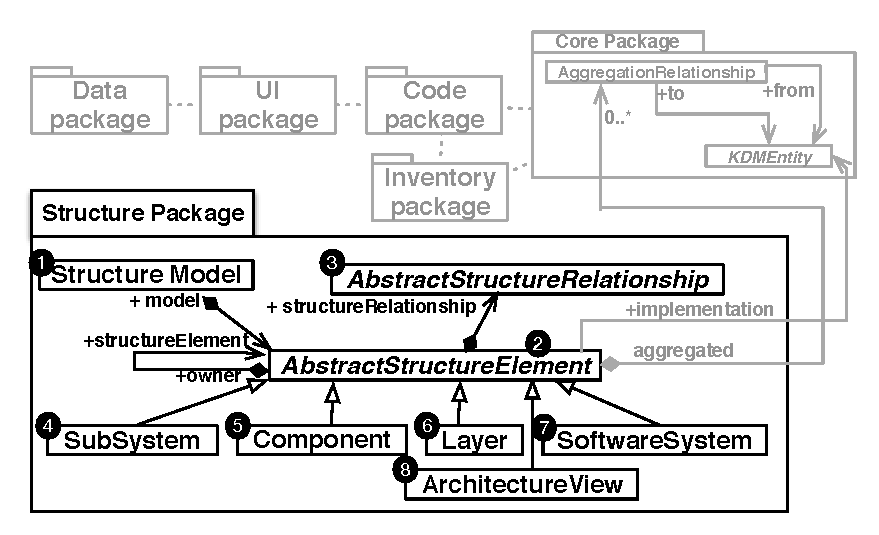
\includegraphics[scale=0.67]{images/StructurePackageFigure}
	\fadaptada{ADM:OMG}
\end{figure}

Esse pacote define um ponto de vista arquitetural para um domínio estrutural. As visões de arquitetura com bae no ponto de vista definido pelo pacote \texttt{Strcuture} representam a forma como os elementos estruturais do sistema de software estão relacionados como os módulos definidos em código-fonte, que correspondem ao pacote \texttt{Code} do KDM. Uma parte simplória do pacote \texttt{Structure} é apresentada na Figura~\ref{fig:structureModel} como um diagrama de classes.

 Usando suas metaclasses é possível relacionar todos os elementos estruturais do sistema, juntamente com os elementos computacionais, isto é, pode-se especificar os elementos estruturais do sistema. Na Figura~\ref{fig:structureModel} é mostrado que o pacote \texttt{Structure} e suas metaclasses são usadas em combinação com os pacotes \texttt{Code}, \texttt{Data}, \texttt{Platform}, \texttt{UI} e \texttt{Inventory}. O modelo \texttt{Structure} possui uma coleção de elementos estruturais, como pode ser visto na Figura~\ref{fig:structureModel} \ding{202}, isso é representado por meio de uma associação. Pacotes (do modelo \texttt{Code}) são os elementos folha do modelo \texttt{Structure}, representando a divisão de um sistema em módulos \texttt{Code} discretos, com partes não sobrepostas. A metaclasse \texttt{SoftwareSystem} fornece um ponto de encontro para todos os pacotes do sistema direta ou indiretamente através de outra associação chamada de \texttt{AbstractStructureElement[0..*]}. Os pacotes podem ainda ser agrupados nas metaclasses \texttt{SubSystem},\texttt{Layer},\texttt{Component} e \texttt{ArchitectureView}. 
 
A metaclasse \texttt{AbstractStructureElement} (conforme a Figura~\ref{fig:structureModel} \ding {203}) representa uma parte arquitetural, relacionada com a organização do sistema de software existente em módulos e possui quatro associações. A primeira associação representa os elementos pertencentes ao modelo e é chamada de $\mathtt{structureElement}$ $\mathtt{:AbstractStructureElement[0..*]}$. Em seguida, há a associação~$\mathtt{structureRelationship}$ $\mathtt{:AbstractStructureRelationship[0..*]}$, ela é usada para representar todas os relacionamentos em nível arquitetural. A associação $\mathtt{aggregated:}$ $\mathtt{AggregatedRelationship[0..*]}$ representa uma relação abstrata entre dois elementos do KDM, dentro dela é possível definir relações concretas. A última associação da metaclasse~$\mathtt{AbstractStructureElement}$ é o~$\mathtt{implementation:KDMEntity[0..*]}$. Esta associação é usada para especificar os elementos computacionais (do pacote~$\mathtt{Code}$, ou seja, $\mathtt{Package}$, $\mathtt{ClassUnit}$, $\mathtt{InterfaceUnit}$, etc) que representam o elemento estrutural. 

Na Figura~\ref{fig:kdm_structureExample} é descrita uma possível arquitetura mostrada para ilustrar como o KDM pode ser utilizado para representar elementos arquiteturais. Pode ser observado que esta figura é dividida em três níveis para ilustrar como o pacote~$\mathtt{Structure}$ está relacionado com o pacote~$\mathtt{Code}$. O nível mais baixo representa o código-fonte, artefatos físicos. L1 e L2 representam pacotes em código-fonte - cada caixa dentro dos pacotes representa as suas classes e interfaces, também é possível perceber que essas classes e interfaces são relacionados uns com os outros de alguma maneira. No meio há metaclasses do pacote~$\mathtt{Code}$, o que significa que as instâncias dessas meta -classes são usadas para representar os artefatos de baixo nível, ou seja, instâncias de~$\mathtt{Package}$ são usadas para representar L1 e L2 e instâncias de~$\mathtt{ClassUnit}$ e~$\mathtt{InterfaceUnit}$ são usados para representar as classes e interfaces, respectivamente. Finalmente, no nível superior a arquitetura é mostrada. Todos os elementos arquiteturais são representados com a seguinte padronização: a metaclasse que representa o elemento arquiteturais, ':' seguido pelo seu nome. A arquitetura apresentada é dividida da seguinte forma: no ponto mais alto de abstração há um~$\mathtt{SoftwareSystem}$ ($\mathtt{S1}$) \ding {202}, que é dividido em duas camadas, ~$\mathtt{Layer}$~$\mathtt{L1}$ \ding {203} e ~$\mathtt{Layer}$~$\mathtt{L2}$ \ding {204}. Tais camadas representam elementos arquiteturais correspondentes aos pacotes L1 e L2 representadas no nível mais baixo. A~$\mathtt{Layer}$~$\mathtt{L1}$ pode acessar os elementos da~$\mathtt{Layer}$~$\mathtt{L2}$, essa restrição \aspas{pode acessar} é representada pela metaclasse~$\mathtt{AggregatedRelationship}$ \ding {205}. Além disso, a~$\mathtt{Layer}$~$\mathtt{L2}$ contém dois componentes,~$\mathtt{C1}$ \ding {206} e~$\mathtt{C2}$ \ding {207}. Finalmente, o~$\mathtt{Component}$~$\mathtt{C1}$ fornece recursos através de uma interface para o~$\mathtt{Component}$~$\mathtt{C2}$.

\noindent \begin{minipage}{.47\textwidth}
	\centering
	\captionof{figure}{Exemplo de uma Arquitetura.}
	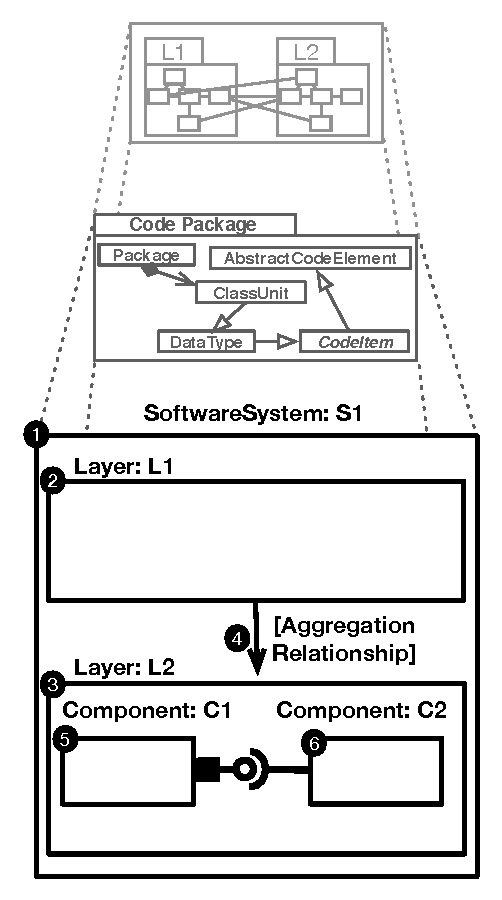
\includegraphics[scale=0.7]{images/StructureExample}
	\fautor
	\label{fig:kdm_structureExample}
\end{minipage}\hfill
\begin{minipage}{.55\textwidth}
	\centering
	\captionof{figure}{Instância KDM correspondente a Figura~\ref{fig:kdm_structureExample}}
	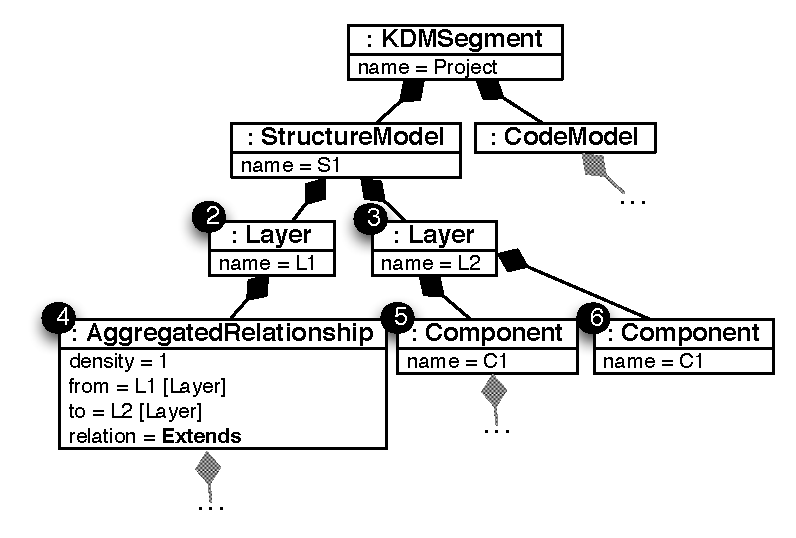
\includegraphics[scale=0.67]{images/StructureKDMINstance}
	\fautor
	\label{fig:kdm_instance_StructureExample}
\end{minipage}


O correspondente, porém simplificado da instância KDM é mostrado na Figura~\ref{fig:kdm_instance_StructureExample}. Os diamantes destacadas em cinza e em anexo com três pontos (\ldots) ilustram que algumas metaclasses não são mostrados de forma a simplificar a figura. Todos os elementos arquiteturais são subclasses de~$\mathtt{StructureModel}$. As camadas são representados pela metaclasse~$\mathtt{Layer}$, como pode ser visto na Figura~\ref{fig:kdm_instance_StructureExample} \ding{203} e \ding{204}. Da mesma forma, os componentes são representados pela metaclasse~$\mathtt{Component}$. A metaclasse mais importante a se destacar nesta figura é $\mathtt{AggregatedRelationship}$. Ela representa a relação entre a $\mathtt{Layer}$ $\mathtt{L1}$ e a $\mathtt{Layer}$ $\mathtt{L2}$. Ela possui meta atributos que tem como objetivo fornecer informações sobre o relacionamento. Por exemplo, o meta atributo~$\mathtt{density}$ ilustra o número de relações primitivas entre estas camadas. Na Figura~\ref{fig:kdm_instance_StructureExample}, o meta atributo~$\mathtt{density}$ possui o valor 1 (um). Outros dois meta atributos são o~$\mathtt{from}$ e o~$\mathtt{to}$, que representam os elementos arquiteturais de origem e destino, respectivamente. Eles são usados para especificar que a~$\mathtt{Layer}$~$\mathtt{L1}$ em~$\mathtt{SoftwareSystem}$~$\mathtt{S1}$ pode acessar a~$\mathtt{Layer}$~$\mathtt{L2}$ também em~$\mathtt{SoftwareSystem}$~$\mathtt{S1}$ de alguma forma. Finalmente, o meta atributo~$\mathtt{relation}$ representa como a~$\mathtt{Layer}$~$\mathtt{L1}$ pode acessar a~$\mathtt{Layer}$~$\mathtt{L2}$, neste contexto, através de herança usando a metaclasse~$\mathtt{Extends}$. Na Figura~\ref{fig:relationship_example_1} é mostrado como as relações entre dois elementos arquiteturais são considerados neste estudo.

\begin{figure}[!ht]
	\centering
	\caption{Relacionamento entre dois elementos arquiteturais}
	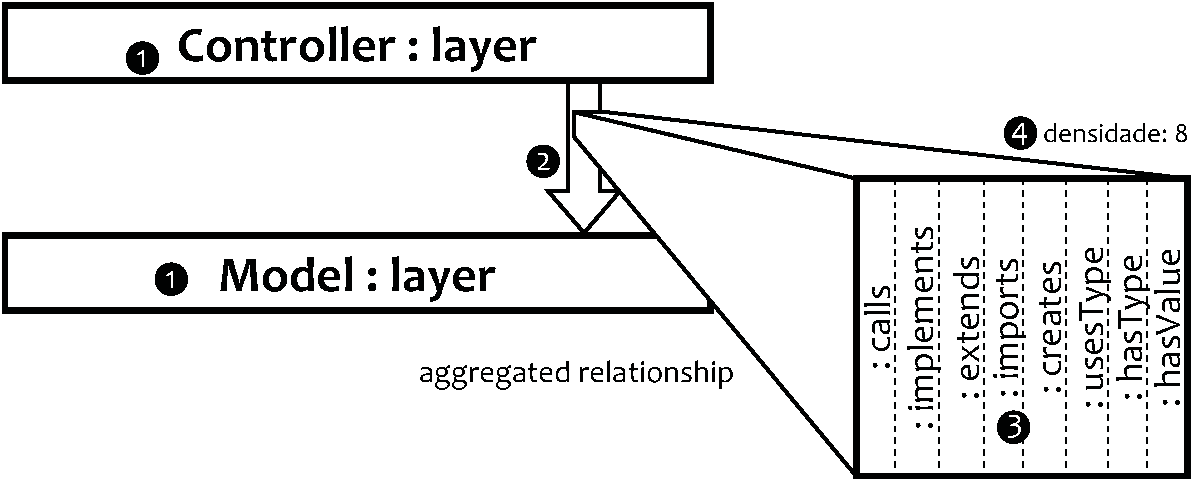
\includegraphics[width=3.3in]{images/relationshipExample1.pdf}
	\fautor
	\label{fig:relationship_example_1}
\end{figure}


Em \ding{202} os elementos arquiteturais são apresentados, camadas~$\mathtt{Controller}$ e~$\mathtt{Model}$. Como visto anteriormente, um relacionamento em nível arquitetural acontece entre dois elementos em nível estrutural (camadas, componentes, subsistemas, etc). Por exemplo, em \ding{203} é mostrando um~$\mathtt{aggregatedRelationship}$ contendo todos os possíveis relacionamentos \ding{204} entre dois elementos (chamadas de métodos, herança, etc). A seta \ding{206} representa o fluxo de entrada e saída dos relacionamentos, em outras palavras, esses relacionamentos representam as possíveis restrições iniciando na camada~$\mathtt{Controller}$  para a camada~$\mathtt{Model}$. Finalmente, a densidade \ding{205} é setada como oito, que representa o número total de relacionamentos possíveis.


\section{Ferramenta de apoio ao KDM}\label{sec:Ferramenta_de_apoio_KDM_capitulo}

Um dos trabalhos mais importantes publicados no contexto da ADM é o de~\citeonline{Bruneliere_2010MODISCO, Bruneliere_2014} que propõe uma ferramenta chamada MoDisco. MoDisco é uma framework genérico e extensível para a abordagem de Engenheria Reversa dirigida a modelos e foi implementada no \sigla{IDE}{\textit{Integrated Development Environment}} Eclipse como um \textit{plugin}. Mais especificadamente, MoDisco é construido utilizando o \textit{Eclipse Modeling Framework} (EMF). Basicamente essa ferramenta é capaz de recuperar o código-fonte legado, base de dados e outros artefatos legado e representá-los com o metamodelo KDM. Um dos principais objetivos da ferramenta MoDisco é ser adaptável para diferentes cenários, facilitando assim a sua utilização por uma base de usuários potencialmente maior~\cite{Bruneliere_2014}. Inicialmente criado como um modelo experimental de investigação pela Equipe AtlanMod (\sigla{EMN}{\textit{Ecole des mines de Nantes}} \& \sigla{INRIA}{\textit{Institut National de Recherche en Informatique et en Automatique}}), o projeto evoluiu para uma solução industrializados graças à colaboração com a empresa MIA-Software. Este trabalho conjunto ativo resultou em um conjunto eficiente e utilizável de ferramentas para a descoberta, consulta e manipulação de modelos de software para auxiliar toda a atividade de engenharia reversa.

MoDisco tem como objetivo representar uma grande variedade de artefatos (por exemplo, código-fonte, banco de dados, arquivos de configuração, documentação, etc.) de um sistema legado. Contudo, uma das limitações dessa ferramenta é o suporte e a aplicação de refatorações. Observe que, naturalmente, MoDisco não é capaz de aplicar refatorações de forma automática, pois a maioria das refatorações necessitam de interação do usuário para fornecer as informações necessárias. No contexto desta Tese foi utilizado a ferramenta MoDisco para recuperar as informações do código-fonte legado escrito em Java. Sem o auxílio dessa ferramenta todo o sistema legado, escrito em Java, deveria ser transformada em uma instância do KDM de forma manual, o que poderia atrasar esta pesquisa, uma vez que toda a manipulação do KDM foi possível por causa da existência do MoDisco e do seu suporte em Java para manipular o metamodelo KDM. Por exemplo, não é possível para o MoDisco adivinhar quais refatorações devem ser aplicadas e em quais elementos; tais informações devem ser fornecidas por um usuário.


%\begin{figure}[!ht]
%	\centering
%	\caption{Visão geral de um projeto MoDisco.}
%	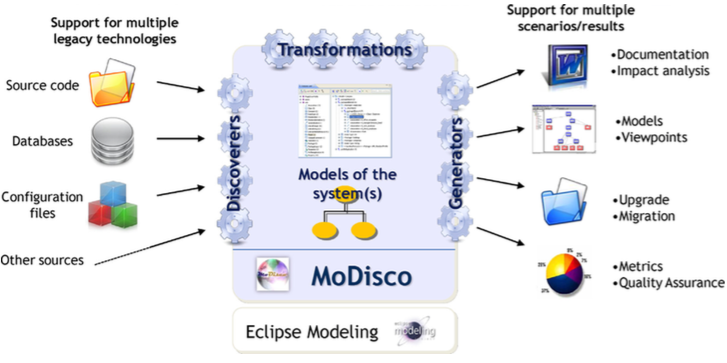
\includegraphics[scale=0.55]{images/modiscoAllArtefacts.png}
%	\label{fig:modisco_allArtefacts}
%	\fadaptada{Bruneliere_2014}
%\end{figure}


\section{Considerações Finais}\label{sec:consideracoes_finais_capitutloADM_KDM}

O foco deste capítulo direciona-se à análise do panorama atual da literatura que trata sobre a modernização de sistemas legados levando em consideração a padronização proposta pelo OMG. Neste capítulo foram mostrados os principais conceitos sobre ADM, KDM, bem como seus pacotes e camadas que são necessários para facilitar o entendimento dessa Tese e fundamentais ao desenvolvimento da proposta aqui desenvolvida.

Observou-se também que o metamodelo KDM por intermédio de suas camadas, pacotes e metaclasses permite a criação de um modelo independente de plataforma que representam um sistema em diversas visões. O objetivo do OMG ao criar esse metamodelo é propor uma padronização da reengenharia de software, fornecendo abstrações que ajudem no processo de reengenharia de sistemas. Além disso, pode-se constatar que diferentemente de metamodelos existentes, tais como a UML, o KDM tem como intuito agrupar todos os artefatos (visões) do sistema em um único metamodelo. Dessa forma, pode-se argumentar que o metamodelo KDM pode ser considerado como uma família de metamodelos, uma vez que o mesmo compartilha uma terminologia consistente e homogenia.

Neste capítulo também foi apresentado sobre a ferramenta MoDisco, uma das principais ferramentas que automatiza a instanciação do metamodelo KDM. Essa ferramenta foi utilizada no contexto deste trabalho para dar suporte à recuperação do modelo KDM a partir de código-fonte legado escrito em Java. No próximo capítulo é apresentado um mapeamento sistemático sobre ADM e KDM.
